%% Springer Nature version of the paper, for the International Journal of
%% Data Science and Analytics (two-column layout, numbered references).
%% GENERATED by scripts/paper_to_springer.py from collusiongraph_paper.tex:
%% edit the IEEE source and regenerate; do not edit this file by hand.
%% Compile beside sn-jnl.cls, sn-mathphys-num.bst, references.bib and figures/.
\documentclass[pdflatex,sn-mathphys-num,iicol]{sn-jnl}
\usepackage{graphicx}
\usepackage{amsmath,amssymb}
\usepackage[title]{appendix}
\usepackage{xcolor}
\usepackage{booktabs}
\usepackage{array}
\graphicspath{{figures/}}
\raggedbottom

\newcommand{\RQ}[1]{\textbf{RQ#1}}
% Revision marker: a number or claim that waits for a named run (revision-plan.md).
\newcommand{\PENDING}[1]{\textcolor{red}{\textbf{[PENDING: #1]}}}
% Author-supplied content that is still missing, or a draft the authors must confirm.
\newcommand{\AUTHORS}[1]{\textcolor{red}{\textbf{[#1]}}}

\begin{document}
\title[One Stack, Two Ledgers]{One Stack, Two Ledgers: Budget-Evaluated, Explainable Collusion Screening Across Illicit-Finance and Procurement Networks}

\author*[1]{\fnm{Rachit} \sur{Garg}}\email{rachit.garg@spjain.org}
\author[1]{\fnm{Kartik} \sur{Joshi}}\email{kartik.as25dxb025@spjain.org}
\author[1]{\fnm{Prem} \sur{Kukreja}}\email{prem.as25dxb029@spjain.org}
\author[1]{\fnm{Gagandeep} \sur{Singh}}\email{gagandeep.as25dxb032@spjain.org}
\author[1]{\fnm{Samuel} \sur{Alex}}\email{samuel.as25dxb031@spjain.org}

\affil*[1]{\orgname{SP Jain School of Global Management}, \orgaddress{\city{Dubai}, \country{United Arab Emirates}}}

\abstract{Money laundering and bid rigging are studied separately, yet both are
collusive crimes. In each, the scheme appears only in the pattern of dealings,
not in any single transaction or tender. We present one graph-learning stack
for both domains: a shared representation, detector family, explanation layer
and evaluation protocol, applied to five public datasets. Under strict
inductive splits and fixed alert budgets, gradient-boosted trees on graph
features outperform every graph neural network we trained on Elliptic++. Over
five seeds, the trees reach an area under the precision--recall curve (AUC-PR)
of $0.8123 \pm 0.0012$, against $0.4729 \pm 0.0525$ for the best graph network,
and the gap holds for every seed pair. The entire gap arises before a market
closure at time step 43, after which both models approach the base rate.
Transfer between procurement markets is uneven: the Garc\'ia markets pool to a
lift of $1.36$ over base rates, the Mendeley countries to $0.93$. Across domains, a frozen procurement encoder reaches $0.150$ AUC-PR on
Elliptic++ (base rate $0.065$), while a linear probe on the target's own
features reaches $0.299$. The reverse direction falls below its base rate. Label noise and
stronger weight decay raise test AUC-PR while lowering validation AUC-PR, so
validation-based selection is unreliable here. The released system ranks group
alerts within a fixed review budget, explains each with a subgraph and a
red-flag citation, and leaves decisions to a human analyst. Code and
configurations are available at
\url{https://github.com/KartikJoshi23/Collusion-Network-Detection}.}

\keywords{graph neural networks, anti-money laundering, bid rigging, anomaly detection, transfer learning, evaluation protocol}

\maketitle


% =====================================================================
\section{Introduction}
% =====================================================================

Money laundering and bid rigging are screened by two enforcement communities
that have never shared a common toolchain. In banks, anti-money-laundering (AML)
teams operate transaction-monitoring rules that fire on individual records.
Most of the resulting alerts are false positives: a CEPS task force reports
that their share is often around 95--98\%~\cite[pp.~3, 31]{lannoo2021}.
Competition authorities and procurement officials face the opposite problem.
Bid-rigging agreements are typically negotiated in secret and are difficult to
detect~\cite[p.~23]{oecd2025}. Detection therefore relies largely on red flags
identified in tenders and on self-reporting through leniency and whistleblower
programmes~\cite[pp.~12, 14]{oecd2025}.

The two problems are closer than they appear. A single small wire transfer
looks unremarkable, whereas twelve accounts passing the same funds around a
cycle within 72 hours constitute a laundering pattern. Likewise, a single bid
can be entirely regular: the tender was advertised, the bids arrived and a
winner was declared. Yet five firms that take turns winning, whose losing bids
lie suspiciously close in price and who share directors and an address, may
form a cartel. In both settings each record appears legitimate in isolation,
and the participants keep every record below the thresholds that the rules
inspect. The scheme becomes visible only in the network of dealings, and
confirmed cases are rare relative to the volume of legitimate activity.

Fig.~\ref{fig:ledgers} illustrates this correspondence. Five mechanisms recur
across the two domains, and each reduces to a single graph signature.
Laundering cycles and bid rotation both appear as directed cycles, smurfing and
cover bidding as fan-in stars, and layering and market allocation as fan-out
stars. Shell-company chains and shared directorships form dense subgraphs of
common attributes, while pass-through clusters and closely grouped bid prices
form tight communities with unusual edge attributes. If this correspondence
holds, a single model can serve both ledgers, and whether a learned notion of
collusive structure transfers between them can be measured rather than
assumed.


\begin{figure*}[t]
\centering
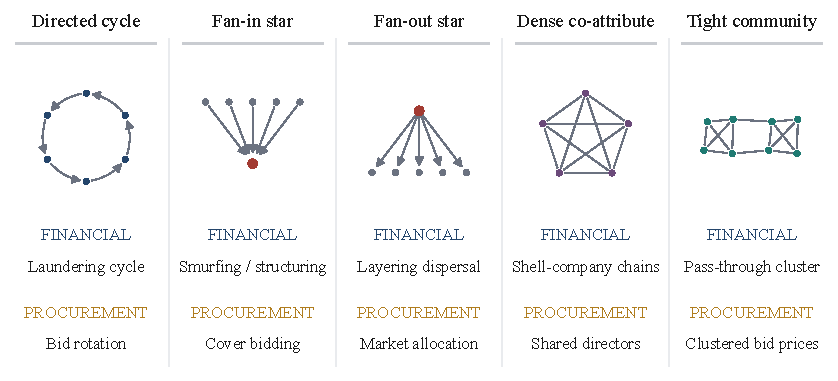
\includegraphics[width=\textwidth]{fig2_two_ledgers.pdf}
\caption{Two ledgers, one structure: five collusion mechanisms, the graph
signature each leaves behind, and its domain-specific name on either side. This
correspondence is the premise of the shared stack, in which only the adapters
and the red-flag vocabularies differ between domains.}
\label{fig:ledgers}
\end{figure*}

Screening tools in both domains are also held to a rising standard of
accountability. For high-risk AI systems, the EU AI Act requires automatic
logging, sufficient transparency for deployers to interpret the output, and
effective human oversight~\cite[Arts.~12--14]{aiact}. For stand-alone
Annex~III systems, these requirements apply from 2~December
2027~\cite{omnibus}. We treat them as the standard that a screening tool should
meet, not as a legal obligation that this system has been shown to face.
Because an AML screener does not assess creditworthiness, it generally falls
outside Annex~III point~5(b)~\cite{aiact,eccguidance}.
Section~\ref{sec:regulatory} maps each requirement onto a property of the
system.

\subsection{Research questions}

\begin{itemize}
\item[\RQ{1}] Can graph neural networks combined with unsupervised graph
anomaly detection identify illicit-finance and bid-rigging structures with
materially higher precision \emph{at fixed alert budgets} than rule-based and
tabular machine-learning baselines?
\item[\RQ{2}] Do models trained on confirmed cases outperform the base rate in
unseen procurement markets, and which planted collusion motifs can
unsupervised detectors recover at a fixed budget?
\item[\RQ{3}] How faithful are the subgraph explanations of the alerts, and
how many alerts match a red-flag pattern that practitioners already use?
\item[\RQ{4}] Does a representation of collusion structure learned in one
domain provide usable signal in the other?
\end{itemize}

\subsection{Contributions}

This paper makes two contributions.

\begin{enumerate}
\item \textbf{A budget-first, leakage-safe evaluation protocol.} It combines
strict inductive splits, frozen train-time normalisation, tie-aware
precision@$k$, multi-seed reporting and paired stratified bootstrap tests. A
leakage test suite enforces the protocol in continuous integration, and a
number-to-config map traces every reported figure to the configuration that
produced it. We regard the protocol as a contribution in its own right because
it implements, rather than merely cites, recent critiques of graph anomaly
evaluation.
\item \textbf{A unified cross-crime representation with transfer
measurements.} A single intermediate representation, populated by six adapters,
holds five public datasets from both domains. Known limitations of each
dataset, such as missing bidder identities, case-control sampling and a
post-window label spike, are recorded explicitly rather than corrected away. On
this representation we measure transfer between procurement markets and
between the two domains.
\end{enumerate}

Two further results support these contributions. The first is a set of
documented negative results, including two five-seed measurements showing that
validation-based model selection cannot detect the distribution shift in
Elliptic++. The second is an explanation layer and a guarded copilot, both
released with the code.

% =====================================================================
\section{Related Work}
% =====================================================================

\textbf{Graph anomaly detection and benchmarks.} The survey by Ma et
al.~\cite{ma2023} provides the node, edge and subgraph taxonomy adopted here.
GADBench~\cite{gadbench} is the most relevant reference point: across 29 models
and ten datasets, tree ensembles with simple neighbourhood aggregation match or
outperform graph neural networks designed for the task. BOND~\cite{liu2022bond}
benchmarks unsupervised detectors in the same manner. Our \RQ{1} result
reproduces this pattern on Elliptic++ under a stricter protocol.

\textbf{AML with graph neural networks.} Motie and Raahemi~\cite{motie2024}
survey the field. LineMVGNN~\cite{linemv2025} adds a line-graph view to two-way
message passing so that the direction of money flow is preserved. On the
original Elliptic data, Weber et al.\ found that a random forest outperformed their graph
convolutional network. They also found that every method, including the random
forest, failed after a dark-market shutdown at time step 43~\cite{weber2019}.
Our \RQ{1} result confirms both findings under a stricter protocol. LaundroGraph
learns self-supervised representations of customer--transaction graphs for
anti-money laundering~\cite{cardoso2022}. Egressy et al.\ extend standard
message passing with reverse message passing, port numbering and ego
identifiers, and report gains of up to 30\% in minority-class F1 on
anti-money-laundering data~\cite{egressy2024}. In our direction-aware graphs,
removing the reverse edges costs $0.194$ AUC-PR, the largest single-component
effect we measured. Near-perfect results on Elliptic are best read alongside the
ablations reported in the same papers. For example, one wavelet-temporal graph
transformer reports an accuracy of about $0.98$~\cite{lin2026}, while noting
that its wavelet features contribute roughly $0.01$ and are ``not strictly
indispensable''.

\textbf{Cartel detection.} Screens based on the coefficient of variation,
price spread and kurtosis of bids are well established and have been tested on
real cartel cases~\cite{imhof2018}. Huber and Imhof combine such screens with
machine learning~\cite{huber2019}, and statistical tests can identify groups of
colluding bidders~\cite{conley2016}. Corruption-risk indicators derived from
procurement records~\cite{fazekas2020} and network analyses of contracting
markets~\cite{wachs2021} extend the approach to corruption more broadly. The
most widely reused benchmarks come from Garc\'ia Rodr\'iguez et
al.~\cite{garcia2022} and the Mendeley EU cartel release~\cite{mendeley2025}.
Recent studies applying graph neural networks to cartels report strong
cross-market results. Graph attention networks over tender--firm graphs from 13 markets in seven
countries transfer with 80--90\% accuracy~\cite{imhof2025}. Their accuracy
peaks at 91\% in an eight-market configuration and settles at 84\% when
extended to 12 markets. Relational GCNs with an explicit zero-shot phase
address out-of-distribution generalisation directly~\cite{gomes2024}. A
systematic mapping study finds that few methods have been applied in real
systems to detect new cases~\cite{epjds2025}. These accuracy figures and our
budget-first lift values are different metrics computed on differently sampled
data, so we make no claim to improve on them. Our transfer matrices instead
characterise how performance degrades. The degradation is uneven across
markets, and on the harder of the two benchmarks the market that fails is the
largest one.

\textbf{Evaluation-protocol critiques.} A recurring criticism is that
machine-learning results, including those on graphs, are inflated by
leakage~\cite{kaufman2012,kapoor2023} and by evaluation on a single fixed
split~\cite{shchur2018}. A third problem is a mismatch between the unit that is
scored and the unit that a human reviews. The disagreement between
transaction-level and actor-level queues in Section~\ref{sec:granularity}
measures this third problem directly.

\textbf{Transfer and graph foundation models.} The literature on graph
foundation models asks whether one representation can serve many
graphs~\cite{liu2025gfm,mao2024}. Pre-training on graph structure can transfer
across graphs~\cite{qiu2020gcc}, but it can also transfer
negatively~\cite{hu2020}. \RQ{4} poses this question for two enforcement
domains in a form that admits a negative answer, and in one direction the
answer is negative.

\textbf{LLM-augmented explanation.} Several groups now combine language models
with graph explanations to produce narratives that an analyst can
read~\cite{cedro2026}. Retrieval grounds generated answers in source
records~\cite{lewis2020}, but hallucination remains a known risk~\cite{ji2023}.
Our assistant is therefore tightly constrained: it issues read-only SQL queries
over the published artifacts, passes every answer through a numeric consistency
check, and screens its output for guilt-attributing language. The aim is an
assistant that supports the reviewer's judgement rather than inviting deference
to it.

% =====================================================================
\section{Data and Unified Representation}
% =====================================================================

\subsection{Datasets}

Table~\ref{tab:data} lists the five public datasets and the six graph views that
our adapters build from them. Elliptic++ supplies both a transaction graph and
an actor graph, and the disagreement between the two is itself a finding
(Section~\ref{sec:granularity}). Two views serve as labelled anchors and carry
the headline results; the others provide scale, controllable ground truth and
an unlabelled population for injection studies. Every dataset is downloaded
from its canonical source and verified against a committed checksum manifest
that also records its licence. No raw data is redistributed in the release.

\begin{table*}[t]
\caption{Five public datasets in the six graph views built by the adapters.
Roles: \textsc{anchor} carries headline results, \textsc{scale} stresses the
pipeline, and \textsc{population} supplies an unlabelled portfolio for
injection. Positives are quoted in each dataset's own unit;
Section~\ref{sec:prevalence} states which denominator each evaluation uses.}
\label{tab:data}
\centering
\footnotesize
\setlength{\tabcolsep}{2.5pt}
\begin{tabular}{llllll}
\toprule
Dataset & Domain & Scale & Positives & Role & Licence \\
\midrule
Elliptic++ (tx graph)~\cite{elmougy2023,weber2019} & Financial & 203,769 nodes, 234,355 edges, 49 steps & $\approx$2\% illicit & \textsc{anchor} & research use \\
Elliptic++ (actor graph)~\cite{elmougy2023} & Financial & test window: 292,102 wallets, 966,352 edges & 5.3\% (test window) & granularity & research use \\
IBM AMLworld HI-Small~\cite{altman2023} & Financial & 5,078,345 tx, 515,088 accounts & 0.102\% laundering & \textsc{scale} & CDLA-Sharing-1.0 \\
Mendeley EU cartel~\cite{mendeleydata2025} & Procurement & 15,616 contracts, 7 countries, 2004--21 & 41.9\% (case-control) & \textsc{anchor} & CC BY-NC 3.0 \\
Garc\'ia Rodr\'iguez et al.~\cite{garcia2022} & Procurement & 64,348 bids, 9,781 tenders, 6 markets & 11.3--81.8\% by market & transfer & CC BY-NC-ND 4.0 \\
OCDS Georgia (OpenTender) & Procurement & 163,327-node window & unlabelled & \textsc{population} & CC BY-NC-SA 4.0 \\
\bottomrule
\end{tabular}
\end{table*}

\subsection{The intermediate representation}

Every adapter emits the same typed structure: nodes, directed attributed edges,
labels with provenance and confidence, and a history pack that supports as-of
feature computation. Everything downstream is therefore domain-agnostic. The
contract also rules out aggressive data cleaning: an adapter may not impute a
missing identity, invent an edge or silently drop an inconvenient property of
the source. As a result, three such properties are preserved in the
representation.

\begin{itemize}
\item \textbf{Garc\'ia bidder identities exist for four of six markets.} The
company-identifier column appears only in the per-market files for Japan, Italy,
Brazil and the USA; the combined file omits it, and the two Swiss markets never
carried it. Co-bidding \emph{identity} graphs can therefore be built for four
markets only, and the remaining markets support only the anonymous bid-price
tier.
\item \textbf{Mendeley is a case-control research sample}, not a population
file, and 41.9\% of its contracts are cartel-linked. Raw AUC-PR therefore
cannot be compared across its folds, whose prevalences range from $0.29$ to
$0.89$. Throughout this paper, the cross-fold comparator is lift over fold
prevalence, never raw AUC-PR.
\item \textbf{AMLworld has a post-window label spike.} Of the 1,108
transactions dated after 10 September, 59.1\% are laundering, roughly 580 times
the base rate. Our temporal splitter excludes this tail explicitly; a naive
split would produce a strikingly high but meaningless score.
\end{itemize}

\subsection{A note on which prevalence is being quoted}
\label{sec:prevalence}

Three different denominators circulate in the literature on these datasets,
and confusing them can make a result appear better or worse than it is. We
therefore fix the convention here and use it throughout the paper.

For Elliptic++, about 2\% of all transactions are labelled illicit, but 77\%
carry no label at all. We compute every metric over confirmed nodes only, and in
the test window of steps 35--49 the confirmed-only prevalence is $0.065$. This
is the baseline against which our AUC-PR should be read, and it is the figure
quoted in Table~\ref{tab:t1}. The 2\% describes the dataset, whereas $0.065$
describes the evaluation.

AMLworld differs by unit rather than by labelling. Laundering accounts for
0.102\% of transactions, while the account-level node prevalence in our test
split is $0.0103$. Because our baselines score accounts, $0.0103$ is the
relevant baseline in Section~\ref{sec:robustness}.

Mendeley differs in the same way. Cartel-linked contracts make up 41.9\% of the
case-control sample, whereas the firm-level test prevalence is $0.358$. Every
Mendeley result we report is at the firm level.

\subsection{As-of label and feature policies}

Any feature computed from a node's history is computed as of the split
boundary, never over the full record. We treat this as part of the evaluation
protocol rather than as an implementation detail, because history-derived
features are where temporal leakage is most likely to hide. Aggregate
statistics do not reveal such leakage; its only symptom is a validation score
that is slightly too good. A dedicated leakage suite enforces these policies
and runs as a separate continuous-integration step on every push.

% =====================================================================
\section{Method}
% =====================================================================

Fig.~\ref{fig:arch} shows the complete system. A single design rule governs it:
a strict trust boundary. The offline pipeline writes plain files and
terminates, and everything on the user-facing side is read-only, so it can
neither retrain a model nor alter a score.

\begin{figure*}[t]
\centering
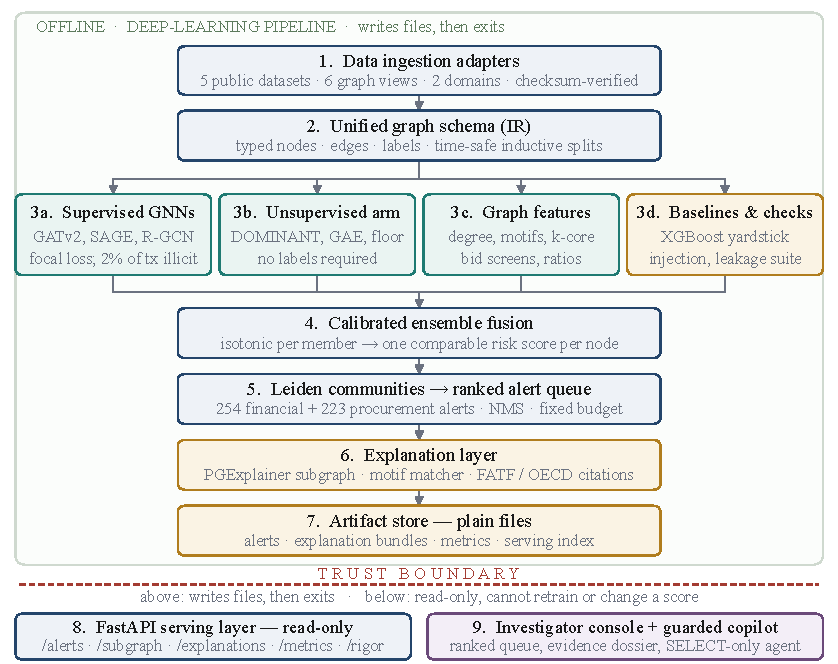
\includegraphics[width=\textwidth]{fig1_architecture.pdf}
\caption{The shared stack. Stages 1--7 run offline and terminate, writing
Parquet and JSON artifacts; stages 8--9 serve those artifacts read-only. The
same nine stages run for both domains; only the ingestion adapters and the
red-flag vocabularies differ.}
\label{fig:arch}
\end{figure*}

\subsection{Detection arms}

Four detection arms score every node, and their scores are fused afterwards.

\textbf{Baselines.} B1 is a rule engine modelled on the threshold logic that
banks deploy in practice. B2 is XGBoost~\cite{chen2016} on node features, and B3
is XGBoost on node features together with graph-derived features: degrees,
k-core, motif counts and neighbourhood aggregates. B3 follows the GADBench
recipe and is the principal yardstick. On the procurement side we add B4, a
transparent composite of award screens: a firm's number of awards, its market
share and the concentration of its buyers. The bid-price screens of the cartel
literature require losing bids, which the Mendeley release does not contain.

\textbf{Supervised graph neural networks.} We use GraphSAGE~\cite{sage},
GATv2~\cite{gatv2} and R-GCN~\cite{rgcn}, all direction-aware: the graph is
built with explicit reverse edges so that message passing can distinguish
sending from receiving. Given the class imbalance, focal loss~\cite{focal} is
the default, and weighted cross-entropy serves as the ablation arm.

\textbf{Unsupervised arm.} DOMINANT~\cite{dominant} and a graph
autoencoder~\cite{kipf2016} score structural reconstruction error, complemented
by a deterministic structural floor. These detectors require no labels and are
the only arms available on the unlabelled OCDS population~\cite{ocds}.

\textbf{Fusion.} We calibrate each member isotonically~\cite{zadrozny2002} on
the validation set before fusion, so that the combined score behaves like a
comparable probability rather than an arbitrary blend of ranks. The difference
between calibrated and rank fusion turned out to be one of the largest effects
measured in this study.

\subsection{From node scores to an alert queue}

The binding constraint for a compliance team is investigator time, not model
output, so the operational unit must be a group rather than a node. Leiden
community detection~\cite{leiden} on the scored graph proposes candidate groups.
We then rank the groups by aggregate member risk, deduplicate them with Jaccard
non-maximum suppression, cap their size and cut the list at a fixed review
budget. A group counts as a hit when at least one member is confirmed illicit.
Precision@$k$ is tie-aware for both nodes and groups: tied scores are counted in
expectation over a random order. Section~\ref{sec:robustness} tests how
sensitive the queue is to the suppression threshold and to the hit rule.

\subsection{Explanation layer}

For each alert the system returns four items. The first is the minimal
responsible subgraph from PGExplainer~\cite{pgexplainer}, which we adopted over
GNNExplainer~\cite{gnnexplainer} after the ablation in Section~\ref{sec:rq3}.
The others are the matched motif, the attributes that support it, and the FATF
or OECD red-flag indicator to which the pattern corresponds. An alert without
an explanation is not considered delivered.

\subsection{Guarded copilot}

A bounded language-model agent answers analyst questions from the published
artifacts and is constrained by design. It has a SELECT-only allowlist over
read-only views and a numeric check that rejects any figure absent from the
rows it has read. It also has a guard against guilt-attributing language and
attaches a disclaimer to every response. Its release gate is a golden set of 26 cases, graded for
grounding and for violations in the released output. Released output has zero
tolerance for violations, while drafted rewrites are held to a separate
limit.

\subsection{Evaluation protocol}
\label{sec:protocol}

Each rule below changed a headline number at some point during development,
which is why we treat the protocol as a result in its own right.
Appendix~\ref{app:methods} gives every split, feature, rule and
hyperparameter.

\begin{itemize}
\item \textbf{Strict inductive splits.} Test nodes and their edges remain
unseen during training. Temporal splits fence the boundary in time, and entity
splits (LOCO, LOMO) hold out entire countries or markets.
\item \textbf{Frozen train-time normalisation.} We compute feature statistics
on the training data and freeze them. Recomputing them on the test graph would
amount to test-time adaptation, because it uses the unlabelled test features.
The effect is large: re-scoring the five stored GATv2 checkpoints with
test-graph statistics raises AUC-PR from $0.4729 \pm 0.0525$ to
$0.6853 \pm 0.0052$ (paired bootstrap, $p \leq 0.001$ on every seed). The entire
gain falls in steps 35--42, from $0.574$ to $0.804$, and after the step-43
closure neither version recovers ($0.039$ and $0.038$). Even with this
adaptation, GATv2 remains below the trees, which use raw features. Every figure
we report uses frozen statistics.
\item \textbf{Budget-first, tie-aware metrics.} We report tie-aware
precision@$k$ at budgets that a real team would use. We also report AUC-PR, the
appropriate summary at this level of class imbalance~\cite{saito2015}, always
read against the prevalence of the corresponding fold.
\item \textbf{Multi-seed with dispersion.} Results are reported over five seeds
as mean~$\pm$~standard deviation. The seed variance, about $\pm 0.05$, is much
larger than the cross-machine variance of about $\pm 0.02$, so a single-seed
comparison between two machines is unreliable. Our earlier project report and
public repository quoted the seed-0 GATv2 figure of $0.5492$, which happens to
be the best of the five seeds. The more reliable figure is the five-seed mean
of $0.4729 \pm 0.0525$, which is the one we report.
\item \textbf{Paired stratified bootstrap}~\cite{efron1993} with 2,000
resamples over identical confirmed test nodes, for every headline
comparison.
\end{itemize}

% =====================================================================
\section{Results}
% =====================================================================

\subsection{RQ1: graph neural networks do not outperform the tree baselines}
\label{sec:rq1}

The answer to \RQ{1} is no. On neither anchor dataset, and at none of the
reported budgets, does a graph neural network, alone or fused with unsupervised
detectors, outperform the tree baselines.

Table~\ref{tab:t1} reports the Elliptic++ results. Gradient-boosted trees on
graph features reach $0.8123 \pm 0.0012$ AUC-PR over five seeds, against a
prevalence of $0.065$, whereas the best graph neural network we trained reaches
$0.4729 \pm 0.0525$. Pairing each GATv2 seed with the tree seed of the same
index, the paired bootstrap places the five differences between $-0.264$ and
$-0.391$. Every 95\% interval lies below zero, and every $p$ value sits at the
resolution floor (Table~\ref{tab:t3}). On scores averaged over the five seeds,
the difference is $-0.301$ (95\% CI $[-0.324, -0.276]$).

\begin{table}[t]
\caption{Elliptic++ node-level results (test steps 35--49, prevalence
$0.065$). The rule baseline is deterministic; tree, GNN and ensemble rows are
5-seed mean $\pm$ standard deviation. The two ``local'' rows use only the 94
local columns (the time step and 93 local features).}
\label{tab:t1}
\centering
\footnotesize
\setlength{\tabcolsep}{4pt}
\begin{tabular}{lll}
\toprule
Model & AUC-PR & P@100 \\
\midrule
B1 rules & 0.0576 (det.) & 0.00 \\
B2 XGBoost, local & $0.7879 \pm 0.0011$ & $1.00 \pm 0.00$ \\
B3 XGBoost + graph, local & $0.7959 \pm 0.0014$ & $1.00 \pm 0.00$ \\
B2 XGBoost & $0.8039 \pm 0.0017$ & $1.00 \pm 0.00$ \\
\textbf{B3 XGBoost + graph} & $\mathbf{0.8123 \pm 0.0012}$ & $\mathbf{1.00 \pm 0.00}$ \\
GATv2-focal & $0.4729 \pm 0.0525$ & $0.8120 \pm 0.2383$ \\
GATv2-weighted CE & $0.4388 \pm 0.0505$ & $0.7240 \pm 0.1466$ \\
DOMINANT & $0.0410 \pm 0.0003$ & --- \\
Ensemble, calibrated & $0.4434 \pm 0.0501$ & --- \\
Ensemble, rank & $0.0511 \pm 0.0019$ & --- \\
Structural floor & $0.0547 \pm 0.0000$ & --- \\
GAE & $0.0386 \pm 0.0001$ & --- \\
\bottomrule
\end{tabular}
\end{table}

\begin{table}[t]
\caption{Paired-bootstrap comparisons over identical confirmed test nodes
($n = 16{,}670$; 2,000 stratified resamples). ``Seed pairs'' rows give the
range of the five per-seed differences and the envelope of their intervals.
``Seed-averaged'' rows compare each model's score averaged over seeds 0--4.
Every $p$ value sits at the resolution floor of 2,000 resamples under add-one
smoothing ($2/2001 \approx 0.001$), so they should be read as $p < 0.001$
rather than as point estimates.}
\label{tab:t3}
\centering
\footnotesize
\setlength{\tabcolsep}{3pt}
\begin{tabular}{lrrr}
\toprule
Comparison & $\Delta$ AUC-PR & 95\% CI & $p$ \\
\midrule
\multicolumn{4}{l}{\textit{GATv2-focal vs.\ B3}} \\
\quad Seed pairs & $-0.264$ to $-0.391$ & $[-0.416, -0.238]$ & $<0.001$ \\
\quad Seed-averaged & $-0.301$ & $[-0.324, -0.276]$ & $<0.001$ \\
\multicolumn{4}{l}{\textit{Calibrated vs.\ rank fusion}} \\
\quad Seed pairs & $+0.342$ to $+0.471$ & $[0.314, 0.500]$ & $<0.001$ \\
\quad Seed-averaged & $+0.444$ & $[0.413, 0.474]$ & $<0.001$ \\
\bottomrule
\end{tabular}
\end{table}

Most of the trees' strength lies in the local transaction features. On the 94
local columns alone, B2 reaches $0.7879 \pm 0.0011$, and the 72 neighbourhood
aggregates and 17 Elliptic++ additions, which include in- and out-degree, add a
further $0.016$. Explicit graph features contribute about $0.008$ in both
settings: B3 outperforms B2 on every seed, and B3-local outperforms B2-local by
the same margin. The graph therefore carries some signal for the trees, but the
deep models fail to convert it into ranking quality, and their deficit appears
before the market closure discussed below.

Calibration matters only once members are fused. Rank fusion of the ensemble
members collapses to $0.0511 \pm 0.0019$, whereas calibrated fusion reaches
$0.4434 \pm 0.0501$ (Table~\ref{tab:t1}). Calibrated fusion is therefore
necessary when members are fused, but it does not outperform its best member:
GATv2-focal alone scores $0.4729 \pm 0.0525$. GATv2 is the only supervised
member of the fusion, and removing the unsupervised members raises the ensemble
by $0.0295$ (Table~\ref{tab:t7}). Adding B3 to a calibrated fusion does not help
either. In that configuration B3 must be trained on steps 1--29 so that steps 30--34
can fit its calibrator. Alone, it then scores $0.8012 \pm 0.0034$; fused with
GATv2, it scores $0.7760 \pm 0.0014$, again below its best member.

Fig.~\ref{fig:crater} shows how the graph model's performance evolves over the
test window. Through step 42 the model remains well above prevalence, but from
step 43 onward it drops to the floor. Step 43 marks the closure of a dark market in the Elliptic timeline, a change
noted since the dataset's original release~\cite{weber2019}. The test window
therefore contains a regime that training never observed. The trees collapse at the same step (Table~\ref{tab:t1b}), as
every method did in the original study~\cite{weber2019}. In steps 35--42, B3
reaches $0.9259 \pm 0.0011$ against $0.5737 \pm 0.0623$ for GATv2, at a
prevalence of $0.092$. In steps 43--49 the prevalence drops to $0.025$, and both
models fall close to it: B3 to $0.0567 \pm 0.0034$ and GATv2 to
$0.0391 \pm 0.0041$. The gap between trees and graph models therefore lies in
steps 35--42, before the closure, and the closure itself defeats both model
families.

\begin{figure}[t]
\centering
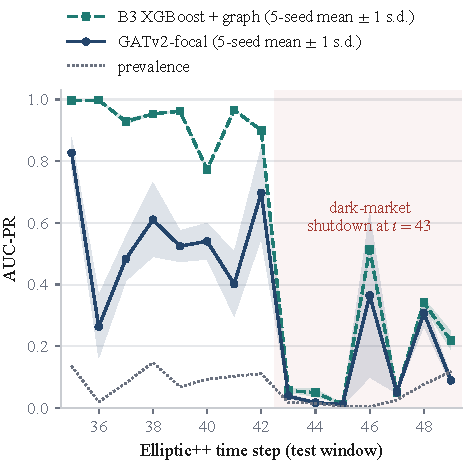
\includegraphics[width=\columnwidth]{fig3_timestep_crater.pdf}
\caption{Per-time-step AUC-PR across the Elliptic++ test window for
GATv2-focal and B3: five-seed means, with shaded bands of one sample standard
deviation. Both models perform well through step 42 and fall towards the
prevalence floor at step 43, when the market closure occurs. A single aggregate
figure conceals this pattern.}
\label{fig:crater}
\end{figure}

\begin{table}[t]
\caption{AUC-PR before and after the step-43 market closure (5 seeds, mean
$\pm$ standard deviation). Each window is scored on its own confirmed test
nodes.}
\label{tab:t1b}
\centering
\footnotesize
\setlength{\tabcolsep}{4pt}
\begin{tabular}{lrrll}
\toprule
Steps & $n$ & Prev. & GATv2-focal & B3 \\
\midrule
35--42 & 9,983 & 0.092 & $0.5737 \pm 0.0623$ & $0.9259 \pm 0.0011$ \\
43--49 & 6,687 & 0.025 & $0.0391 \pm 0.0041$ & $0.0567 \pm 0.0034$ \\
\bottomrule
\end{tabular}
\end{table}

The procurement anchor (Table~\ref{tab:t2}) preserves the same ordering and is
even less favourable to the graph model. R-GCN scores $0.2808 \pm 0.0087$
against a prevalence of $0.358$, a result that is stable across seeds and below
the base rate. This is not a label or score inversion: the labels map
correctly, and the inverted scores reach $0.43$ to $0.47$ on every seed. The
cause is a reversal over time. The training firms are 87--89\% cartel-linked, against 36\% in the test set.
Among firms first seen up to 2010, where the R-GCN computes its loss, every
usable structural feature ranks licit firms above cartel firms. Degree, for example, has a ROC-AUC of $0.38$ for the label in that period and
$0.61$ in the test set. A model fitted on that window therefore ranks the test
firms in reverse. Its validation AUC-PR of $0.94$ to $0.95$ lies just above
the validation prevalence of $0.89$, so validation cannot reveal the problem.
Removing the two component-size features, which shift most between the
periods, does not help ($0.2997 \pm 0.0015$).

The best tree model is XGBoost with the publisher's precomputed screens added,
at $0.4547 \pm 0.0081$. A linear probe on the seven award screens reaches
$0.4752$ on the same test firms (Table~\ref{tab:fulllabel}), above every tree.
On this dataset, therefore, the established screening approach contributes more
than the graph model does.

\begin{table}[t]
\caption{Mendeley EU firm-level results (within the case-control sample,
prevalence $0.358$), to be read as lift over prevalence. Rule and screen rows
are deterministic; tree and R-GCN rows are 5-seed mean $\pm$ standard
deviation. ``+screens'' rows add the publisher's own precomputed screen columns
to that baseline's inputs.}
\label{tab:t2}
\centering
\footnotesize
\setlength{\tabcolsep}{4pt}
\begin{tabular}{lll}
\toprule
Model & AUC-PR & P@18 \\
\midrule
B1 rules & 0.3426 (det.) & 0.47 \\
B2 XGBoost & $0.3849 \pm 0.0099$ & $0.22 \pm 0.00$ \\
B3 XGBoost + graph & $0.3749 \pm 0.0092$ & $0.57 \pm 0.06$ \\
B4 screens & 0.3811 (det.) & 0.78 \\
\textbf{B2 + screens} & $\mathbf{0.4547 \pm 0.0081}$ & $0.66 \pm 0.06$ \\
B3 + screens & $0.3509 \pm 0.0058$ & $0.20 \pm 0.03$ \\
B4 + screens & 0.3874 (det.) & 0.50 \\
R-GCN focal & $0.2808 \pm 0.0087$ & $0.07 \pm 0.04$ \\
\bottomrule
\end{tabular}
\end{table}

\subsection{Queue granularity: the scored unit is not the reviewed unit}
\label{sec:granularity}

Scoring transactions and scoring actors turn out to be different problems, and
the difference is visible in the results. On the Elliptic++ actor graph, R-GCN
reaches $0.3400 \pm 0.0632$ AUC-PR over five seeds against a prevalence of
$0.053$, a lift of $6.4\times$. Although the seeds range from $0.2473$ to
$0.4033$, the head of the ranking is stable: precision@100 is $0.98$ for seed 0
and $1.00$ for the other four. When these node scores are aggregated into review
groups, however, queue precision collapses. The 2,514 actor alerts from the
seed-0 model reach a precision@50 of $0.08$, and over the five seeds the queue
reaches $0.14 \pm 0.03$, compared with $0.99$ for the node ranking.

The transaction-level queue, built from the seed-0 calibrated ensemble, behaves
in the opposite way. Its 318 communities condense into 254 alerts with a
precision@50 of $0.32$, a precision@100 of $0.25$ and a precision@200 of
$0.135$. This is a usable triage list, and its top 50 alerts cover 7.9\% of the
illicit population. The procurement queue, built from the seed-0 R-GCN, yields 223 alerts from
1,283 communities but barely ranks them. Its top 129 alerts share a single
calibrated score, so its precision@18 of $0.40$ is close to the $0.39$ obtained
by ordering the same 223 alerts at random.

Node-level ranking quality and queue-level precision are therefore not
interchangeable. Reporting only the former does not establish whether a model
is useful for real-world triage, so we report both.

\subsection{RQ2: unseen markets and planted motifs}
\label{sec:rq2}

\RQ{2} has two parts. The first asks whether a model trained on confirmed cases outperforms the base
rate in a procurement market it has never seen. The second asks which planted
collusion motifs unsupervised detectors can recover.

\textbf{Transfer to unseen markets.} Fig.~\ref{fig:transfer} and
Table~\ref{tab:t4} present the two procurement transfer matrices. Held-out
prevalences range from $0.29$ to $0.89$ across the Mendeley folds and from
$0.25$ to $0.55$ across the Garc\'ia folds. Lift over each fold's own
prevalence is therefore the only fair comparator.

\begin{figure}[t]
\centering
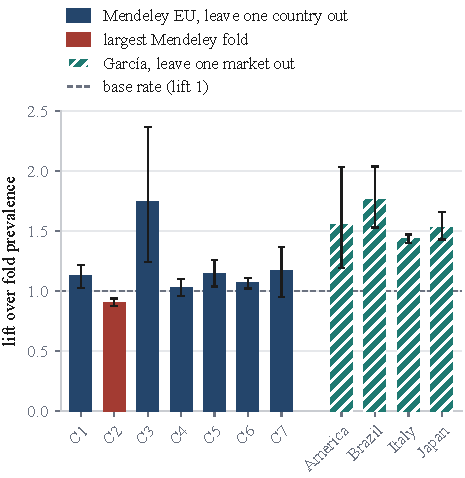
\includegraphics[width=\columnwidth]{fig4_transfer_lift.pdf}
\caption{Transfer lift by held-out fold, with bootstrap 95\% intervals. All
four Garc\'ia markets exceed their base rate under leave-one-market-out
evaluation. On Mendeley's leave-one-country-out folds (C1--C7), the pooled lift
is $0.93$, and the largest fold, C2 with 750 of 1,001 firms, falls below $1.0$.
C1--C7 stand for the release's codes \texttt{country\_1} to
\texttt{country\_7}. A bar at or below $1.0$ indicates no improvement over the
fold's own base rate.}
\label{fig:transfer}
\end{figure}

\begin{table}[t]
\caption{Procurement transfer matrices, 5 seeds per fold. Lift is AUC-PR
divided by the held-out fold's own prevalence; $1.0$ means no better than the
fold's base rate. Fold AUC-PR is the mean $\pm$ standard deviation over seeds;
brackets give a stratified bootstrap 95\% interval (2,000 resamples) on the
seed-averaged scores. Pooled rows score all held-out firms together (mean
$\pm$ standard deviation over seeds). Size-weighted lift weights each fold by
its $n$.}
\label{tab:t4}
\centering
\footnotesize
\setlength{\tabcolsep}{2pt}
\begin{tabular}{lrrll}
\toprule
Held-out fold & $n$ & Prev. & AUC-PR & Lift [95\% CI] \\
\midrule
\multicolumn{5}{l}{\textit{Mendeley EU --- leave-one-country-out}} \\
\quad country\_1 & 30 & 0.77 & $0.8664 \pm 0.0224$ & 1.13 [1.03, 1.22] \\
\quad country\_2 & 750 & 0.72 & $0.6464 \pm 0.0182$ & 0.90 [0.87, 0.94] \\
\quad country\_3 & 63 & 0.29 & $0.4983 \pm 0.0603$ & 1.74 [1.24, 2.36] \\
\quad country\_4 & 76 & 0.72 & $0.7427 \pm 0.0812$ & 1.03 [0.96, 1.10] \\
\quad country\_5 & 60 & 0.67 & $0.7630 \pm 0.0473$ & 1.14 [1.04, 1.26] \\
\quad country\_6 & 9 & 0.89 & $0.9527 \pm 0.0346$ & 1.07 [1.02, 1.11] \\
\quad country\_7 & 13 & 0.69 & $0.8091 \pm 0.0060$ & 1.17 [0.95, 1.36] \\
\quad Pooled & 1,001 & 0.69 & $0.6404 \pm 0.0153$ & $0.93 \pm 0.02$ \\
\quad Size-weighted & & & & 0.99 \\
\midrule
\multicolumn{5}{l}{\textit{Garc\'ia Rodr\'iguez --- leave-one-market-out}} \\
\quad USA & 120 & 0.25 & $0.3894 \pm 0.1080$ & 1.56 [1.19, 2.03] \\
\quad Brazil & 272 & 0.29 & $0.5063 \pm 0.1161$ & 1.77 [1.53, 2.04] \\
\quad Italy & 821 & 0.55 & $0.7858 \pm 0.0585$ & 1.43 [1.40, 1.47] \\
\quad Japan & 1,665 & 0.28 & $0.4295 \pm 0.0223$ & 1.53 [1.43, 1.66] \\
\quad Pooled & 2,878 & 0.36 & $0.4827 \pm 0.0544$ & $1.36 \pm 0.15$ \\
\quad Size-weighted & & & & 1.53 \\
\midrule
\multicolumn{5}{l}{\scriptsize Macro lift (unweighted mean of the fold
lifts): $1.17$ Mendeley, $1.57$ Garc\'ia.} \\
\bottomrule
\end{tabular}
\end{table}

All four Garc\'ia markets exceed their own base rate under leave-one-market-out
evaluation, and every per-fold 95\% interval for lift lies above 1. Pooled over
all held-out firms, the lift is $1.36 \pm 0.15$ across seeds; weighted by fold
size, it is $1.53$. The Italy fold is strong enough that a three-alert queue
built on it returns three confirmed cartels. Leave-one-country-out transfer on
Mendeley is considerably weaker. \texttt{country\_2} holds 750 of the 1,001
held-out firms and reaches a lift of $0.90$ (95\% CI $[0.87, 0.94]$), below its
own base rate. Pooled over all firms, the Mendeley lift is $0.93 \pm 0.02$, and
weighted by size it is $0.99$. Only four folds have an interval above 1, and
together they hold 162 firms, so the macro lift of $1.17$ is driven by small
folds. The data release names the seven countries but does not specify which
code corresponds to which country~\cite{mendeley2025}, so the folds retain
their codes.

\textbf{Planted motifs.} Because confirmed cartels are scarce, we plant known
motifs into the unlabelled 163,327-node OCDS Georgia window and measure their
recovery at a fixed budget. Only the unsupervised arms can run without labels,
so this experiment measures how detectable each planted motif is, not what a
supervised model learns from it. Table~\ref{tab:t6} shows a clear difference
between two types of motif.
\label{sec:injection}

\begin{table}[t]
\caption{Injected-member recall@2000 on the OCDS Georgia window (population
163,327; 5 seeds, mean $\pm$ s.d.; rank-fusion unlabelled mode, since the
unsupervised arms are the only ones available without labels). The dispersion
is wide for the two recovered families: the seed-to-seed spread exceeds several
of the between-method differences.}
\label{tab:t6}
\centering
\footnotesize
\setlength{\tabcolsep}{1.5pt}
\begin{tabular}{lllll}
\toprule
Motif family & DOMINANT & Ens.\ (rank) & Floor & GAE \\
\midrule
Coordinated cluster & $0.37 \pm 0.15$ & $\mathbf{0.92 \pm 0.17}$ & $0.12 \pm 0.00$ & $0.91 \pm 0.12$ \\
Common control & $\mathbf{0.58 \pm 0.04}$ & $0.44 \pm 0.02$ & $0.43 \pm 0.00$ & $0.47 \pm 0.02$ \\
Partition & $0.17 \pm 0.01$ & $0.03 \pm 0.03$ & $0.00 \pm 0.00$ & $0.05 \pm 0.01$ \\
Rotation & $0.08 \pm 0.01$ & $0.00 \pm 0.00$ & $0.00 \pm 0.00$ & $0.04 \pm 0.01$ \\
Cover bid & $0.01 \pm 0.01$ & $0.00 \pm 0.00$ & $0.00 \pm 0.00$ & $0.01 \pm 0.01$ \\
\bottomrule
\end{tabular}
\end{table}

Motifs that change the shape of the graph are detected more easily: coordinated
clusters reach a recall of $0.92$ and common control reaches $0.58$. Motifs that
alter only who wins remain nearly invisible, and rotation, cover bidding and
market partition never exceed $0.17$ under any method we tested. The limitation
is structural and is unlikely to be removed by tuning. Bid rotation leaves the
co-bidding topology essentially unchanged and alters only the award labels
along the edges, so detecting it requires award-sequence features rather than
deeper message passing. We regard this as one of the more useful negative
results reported here, given how often the cartel literature treats rotation as
a characteristic detectable pattern.

One caveat applies. Coordinated-cluster recall has a standard deviation of
$0.17$ over five seeds. The apparent ordering between the rank ensemble at
$0.92$ and the graph autoencoder at $0.91$ therefore lies well within noise. The
experiment supports the family-level distinction between shape-changing and
award-changing motifs, but not a ranking of unsupervised detectors, and we do
not offer one.

\subsection{RQ4: cross-domain transfer is asymmetric and label-dependent}
\label{sec:rq4}

\textbf{Frozen probes.} We freeze an encoder trained on one domain and probe it
on the other. Neither encoder ever ingests raw features. Both domains enter
through the same ten-column structural template, z-scored within each graph,
so the 183 Elliptic++ columns and the procurement screens never reach an
encoder. Table~\ref{tab:fulllabel} compares each frozen probe at full labels
with probes on the target's own inputs, and the two directions disagree. From
financial to procurement, the probe reaches $0.2843$ against a prevalence of
$0.358$, which is below the base rate and therefore carries no signal. Its inverted
scores reach $0.43$, and the labels map correctly. The cause is the temporal
reversal of the Mendeley structural signal described in
Section~\ref{sec:rq1}, not an inversion bug. From
procurement to financial, it reaches $0.1502$ against $0.065$, a lift of $2.3$,
and outperforms a probe on the target's own structural template by $0.042$
(95\% CI $[0.026, 0.059]$). However, a logistic probe on the inputs of B2
reaches $0.2991$ on the same nodes, and B2 itself reaches $0.8039 \pm 0.0017$.
The transferred encoder therefore carries some structural signal, but far less
than the target's own features.

\begin{table}[t]
\caption{Cross-domain probes at full labels, on the published probe's train
and test pools. Each probe is a class-balanced logistic regression: on
embeddings from the stored source encoder (frozen), on the target's own
structural template (structural), or on the inputs of B2 (B2-input). Brackets
give stratified bootstrap 95\% intervals; the B2 row is the 5-seed tree
result.}
\label{tab:fulllabel}
\centering
\footnotesize
\setlength{\tabcolsep}{3pt}
\begin{tabular}{lll}
\toprule
 & Fin.\ $\rightarrow$ proc. & Proc.\ $\rightarrow$ fin. \\
\midrule
Test nodes, prevalence & 363, 0.358 & 16,670, 0.065 \\
Frozen probe & $0.2843$ $[0.268, 0.311]$ & $0.1502$ $[0.135, 0.169]$ \\
Structural probe & $0.2705$ $[0.255, 0.293]$ & $0.1084$ $[0.100, 0.118]$ \\
B2-input probe & $0.4752$ $[0.421, 0.545]$ & $0.2991$ $[0.280, 0.322]$ \\
B2 XGBoost & $0.3849 \pm 0.0099$ & $0.8039 \pm 0.0017$ \\
\bottomrule
\end{tabular}
\end{table}

\textbf{Label efficiency.} Fig.~\ref{fig:labeleff} varies the number of
available target-domain labels, with five draws per budget. Below 1,000
labels, ten of the twelve budgets show a negative transfer gain, and the two
positive gains, both $+0.002$, lie within one standard deviation of zero. At
these budgets the frozen source probe performs no better than a probe trained
on the target's own structural features. From procurement to financial, the
probe gains a clear advantage only from 1,000 labels ($+0.013$) and reaches
$+0.042$ at full labels. In the other direction, no probe's mean AUC-PR reaches
the base rate at any budget. Transfer is therefore a convenience once labels
are plentiful, not a solution to the cold-start problem.

\begin{figure}[t]
\centering
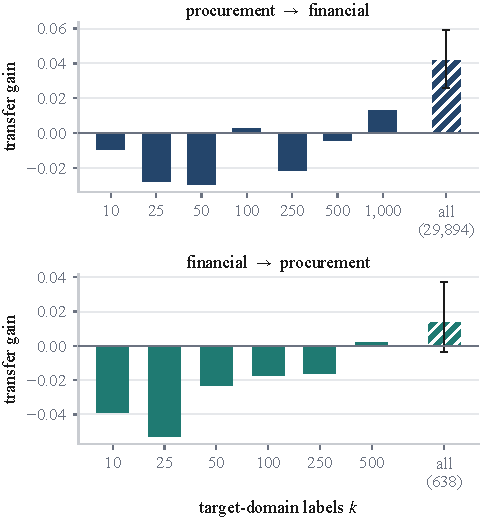
\includegraphics[width=\columnwidth]{fig6_label_efficiency.pdf}
\caption{Cross-domain label efficiency. Each bar gives the gain of a frozen
source-domain probe over a probe trained on the target's own structural
features, at the same label budget (five draws per budget). The hatched bar
uses every training label (Table~\ref{tab:fulllabel}), with its paired
bootstrap 95\% interval. Below 1,000 labels, ten of twelve bars are negative
and the other two lie within one standard deviation of zero. Transfer does not
solve the cold-start problem in either direction.}
\label{fig:labeleff}
\end{figure}

\subsection{Robustness, ablations and validation reliability}
\label{sec:robustness}

Table~\ref{tab:t7} collects the component ablations, which follow two
conventions. A ``$-$'' row removes a component from the adopted model, so its
delta is the cost of removal. A ``$+$'' row adds a variant that we evaluated
but did not adopt, so its delta is a rejection margin. The two are different
measures and should not be compared directly; only the ``$-$'' rows quantify
how much each component contributes. Each delta is measured against the
reference result with the same setup, and no seed-0 result is compared with a
multi-seed mean.

\begin{table}[t]
\caption{Component ablations. ``$-$'' rows are ablation costs; ``$+$'' rows
are rejection margins for variants that were measured and not adopted.}
\label{tab:t7}
\centering
\footnotesize
\setlength{\tabcolsep}{3.5pt}
\begin{tabular}{llll}
\toprule
Arm & Basis & AUC-PR & $\Delta$ \\
\midrule
GATv2-focal (headline) & 5 seeds & $0.4729 \pm 0.0525$ & ref. \\
\quad $-$ focal loss & 5 seeds & $0.4388 \pm 0.0505$ & $-0.0341$ \\
Calibrated ensemble & 5 seeds & $0.4434 \pm 0.0501$ & ref. \\
\quad $-$ unsup.\ members & 5 seeds & $0.4729 \pm 0.0525$ & $+0.0295$ \\
GATv2-focal (headline) & seed 0 & $0.5492$ & ref. \\
\quad $-$ bidir.\ edges & seed 0 & $0.3549$ & $\mathbf{-0.1943}$ \\
\quad $+$ structural chan. & seed 0 & $0.3781$ & $-0.1711$ \\
\quad $+$ line-graph chan. & seed 0 & $0.4986$ & $-0.0506$ \\
\quad $+$ context fusion & seed 0 & $0.3242$ & $-0.2250$ \\
Mendeley B2 XGBoost & 5 seeds & $0.3849 \pm 0.0099$ & ref. \\
\quad $+$ dataset screens & 5 seeds & $0.4547 \pm 0.0081$ & $+0.0698$ \\
\bottomrule
\end{tabular}
\end{table}

Direction-awareness is the most influential component: dropping the reverse
edges reduces AUC-PR by $0.194$. This is consistent with the gains that
Egressy et al.\ report from reverse message passing on a different dataset~\cite{egressy2024}.
Focal loss gives a smaller improvement of $0.034$. Additional input channels
reduced performance in every case: the structural, line-graph and
context-fusion variants all performed worse than the raw features alone. We
interpret this as an interaction between model capacity and distribution
shift, not as evidence that these channels carry no information in
general.


\textbf{Protocol sensitivity.} We swept the Jaccard suppression threshold over
$\{0.3, 0.4, 0.5, 0.6, 0.7\}$, crossed with three hit-rule settings. The two
axes behave differently, so we do not combine them into a single robustness
claim.

Suppression does not change the alert set. At every threshold, the financial
queue keeps all 254 alerts and the procurement queue all 223, with none
suppressed anywhere in the grid. Because the communities barely overlap,
non-maximum suppression has no effect, and the published queues do not depend
on a tuned de-duplication setting.

The hit rule matters more. Our published queue counts a group as a hit when at
least one member is confirmed illicit. A stricter rule requires illicit members
to make up at least $0.1$ of a group's confirmed members. Under it, financial
precision@50 falls from $0.32$ to $0.30$, P@100 from $0.25$ to $0.23$, and P@200 from
$0.135$ to $0.125$. Tightening the fraction further to $0.25$ costs nothing
beyond that. The procurement queue is flat on the suppression axis, and on the
hit-rule axis its P@18 moves from $0.40$ to $0.39$ and then to $0.37$. About
$0.02$ of our headline queue precision therefore rests on a definitional
choice. We report the looser rule and state this dependence explicitly.

\textbf{The label-noise result.} Fig.~\ref{fig:noise} presents the most
striking negative result in the paper. We flipped a fraction of the training
labels at random and tracked validation and test AUC-PR together over five
seeds. Test AUC-PR rose from $0.4729 \pm 0.0525$ on clean labels to
$0.5646 \pm 0.0456$ with 10\% of labels flipped, and remained at
$0.5507 \pm 0.0690$ with 20\%. Over the same range, validation AUC-PR fell from
$0.9380$ to $0.5642$, so the two curves move in opposite directions. At 10\%
every seed outperformed its clean run, and at 5\% and 20\% four of five did.
The clean runs are the headline runs, so the curve starts at the headline
value.

\begin{figure}[t]
\centering
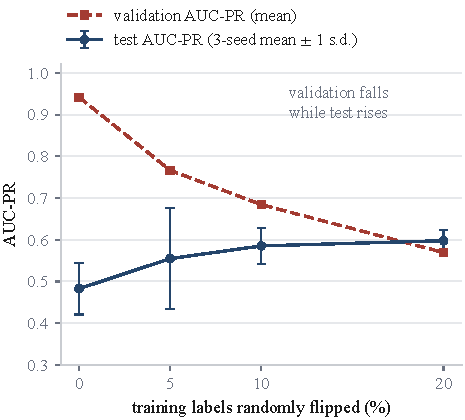
\includegraphics[width=\columnwidth]{fig5_label_noise.pdf}
\caption{Effect of label noise on Elliptic++ (GATv2-focal, five seeds per
rate). Corrupting the training labels \emph{improves} test AUC-PR while
validation AUC-PR collapses, so model selection on validation optimises against
the wrong curve.}
\label{fig:noise}
\end{figure}

The gain falls entirely before the market closure. In steps 35--42, AUC-PR
rises from $0.574$ to $0.683$ with 10\% noise, whereas in steps 43--49 it drops
from $0.039$ to $0.025$, level with the base rate. Noise therefore does not
carry the model across the closure. Instead, it improves performance on the
steps immediately after validation (30--34) while validation performance itself
falls, so the two windows disagree about the same models even before the
break.

\begin{table}[t]
\caption{Label noise against explicit regularisers (GATv2-focal on
Elliptic++, five seeds; test mean $\pm$ standard deviation, validation
mean). Each arm changes one setting of the headline run. The last column
counts the seeds whose test AUC-PR exceeds that of the clean run with the same
seed. The window arm validates on steps 32--34, so its validation value is not
comparable.}
\label{tab:regularisers}
\centering
\footnotesize
\setlength{\tabcolsep}{3pt}
\begin{tabular}{llrr}
\toprule
Arm & Test AUC-PR & Val. & Above clean \\
\midrule
Clean labels (headline) & $0.4729 \pm 0.0525$ & $0.9380$ & --- \\
Label noise 5\% & $0.5493 \pm 0.0870$ & $0.7735$ & 4/5 \\
Label noise 10\% & $0.5646 \pm 0.0456$ & $0.6832$ & 5/5 \\
Label noise 20\% & $0.5507 \pm 0.0690$ & $0.5642$ & 4/5 \\
Label smoothing, $\varepsilon = 0.1$ & $0.4585 \pm 0.0344$ & $0.9387$ & 2/5 \\
Weight decay $5 \times 10^{-3}$ & $0.5403 \pm 0.0286$ & $0.8996$ & 5/5 \\
Dropout 0.5 & $0.4874 \pm 0.0362$ & $0.9419$ & 4/5 \\
Early-stopping patience 5 & $0.4224 \pm 0.0589$ & $0.8913$ & 0/5 \\
Validation on steps 32--34 & $0.4772 \pm 0.0468$ & $0.9583$ & 2/5 \\
\bottomrule
\end{tabular}
\end{table}

Explicit regularisers fall into two groups (Table~\ref{tab:regularisers}).
Weight decay of $5 \times 10^{-3}$, ten times the headline value, behaves like
label noise. Test AUC-PR rises to $0.5403 \pm 0.0286$, above the clean run on
all five seeds, while validation AUC-PR falls to $0.8996$. Its gain also lies
in steps 35--42, from $0.574$ to $0.659$. Dropout raises test AUC-PR slightly
and leaves validation unchanged, whereas label smoothing and a patience of 5
lower test AUC-PR. A later validation window does not help either: trained on
steps 1--31 and validated on steps 32--34, the model scores $0.9583$ on
validation and $0.4772 \pm 0.0468$ on test. Among the eight variants that share
the original validation window, validation would select dropout, which ranks
only fifth on test. Label noise and weight decay are thus the two measurements
in which validation-based selection prefers the setting that performs worse on
test.

These experiments are diagnostic, not training recommendations: they show that
validation-based selection is unreliable under this shift.

\textbf{AMLworld at scale.} For completeness, we report a negative result at the
scale of 5M edges. The tree baselines score $0.0063$ (B2) and $0.0062$ (B3) against an
account-level prevalence of $0.0103$ (Section~\ref{sec:prevalence}), so both
fall below chance. Their inverted scores, by contrast, reach $0.0211$ and
$0.0239$, about twice the prevalence. The labels map
correctly, so this is not an inversion bug; the cause is the split. Accounts
are heavily front-loaded, so a split by first appearance places the training
cut one hour into the data, and the training features see only 344,747 of
5,078,345 transactions. Within that hour the money-flow features carry almost
no label signal (ROC-AUC $0.49$ to $0.54$), whereas over the full window the
same features carry a strong signal (up to $0.74$). The trees therefore learn
from noise, and their splits do not generalise to accounts observed over ten
days. We consequently use AMLworld for its intended purpose, injection against
known ground truth, rather than as a supervised benchmark.

% =====================================================================
\section{Explanation Study}
\label{sec:rq3}
% =====================================================================

\RQ{3} asks how faithful the subgraph explanations are and how many alerts
match a red-flag pattern that practitioners already use. We answer it from
fidelity and coverage measurements on the published queue, and the answer is
mixed. PGExplainer's explanations pass PyG's fidelity sanity check on 49 of 50
alerts, but only 25 of 50 pass a stricter uniform test, and no explainer
produces sparse explanations. On the financial queue, 15 of 50 alerts match a
red-flag pattern; on the procurement queues, none do.

\textbf{Choosing an attribution method.} We ran a three-arm ablation over the
top members of the 50 highest-ranked financial alerts, comparing GNNExplainer,
PGExplainer and raw attention (Table~\ref{tab:explainers}). Each arm keeps the 20 highest-scoring edges of a two-hop window around the node.
Following the standard definitions~\cite{yuan2023,agarwal2023}, Fidelity+
measures how much the model's prediction changes when the explanation is
removed. Fidelity$-$ measures how much it changes when only the explanation is
retained. We call an attribution \emph{sane} when its Fidelity+ is at least its
Fidelity$-$. Removing a sane explanation therefore disturbs the prediction at
least as much as keeping only the explanation does. An explanation bundle whose
attribution is not sane carries an \emph{implausible-fidelity} flag. Under
PyG's fidelity measure~\cite{fey2019}, PGExplainer returned sane attributions for 49
of the 50 nodes, compared with 10 for GNNExplainer, in under a third of the
time. We therefore adopted it. Its bundles carry an implausible-fidelity
flag on 1 of 50 alerts, against 40 of 50 for GNNExplainer.

A uniform test gives a less favourable picture. We remove or retain the selected edges outright, using hard masks, and measure
both fidelities as drops in the model's probability for its own prediction.
Under this test the three arms are close: Fidelity+ ranges from $0.049$ to
$0.052$, and 22 to 25 of the 50 explanations of each arm are sane
(Fidelity+ $\geq$ Fidelity$-$). Sparsity is low
because most two-hop windows contain few more edges than the 20 retained, and
attention keeps almost every edge. The arms also largely agree on which edges
matter, with mean Jaccard overlaps of their edge sets between $0.65$ and
$0.88$. Attention, often favoured because it appears to offer interpretability
at no extra cost~\cite{jain2019}, performs on a par with GNNExplainer under
this test.

\begin{table}[t]
\caption{Explainer metrics on the top members of the 50 highest-ranked
financial alerts (seed-0 GATv2, two-hop windows, 20 kept edges). ``PyG sane''
uses PyG's fidelity measure. Hard-mask Fidelity$\pm$ are mean probability
drops for the model's own prediction; ``hard sane'' counts nodes with
Fidelity+ $\geq$ Fidelity$-$. Sparsity is the share of window edges left out.
Time is wall-clock on one 4-core laptop CPU.}
\label{tab:explainers}
\centering
\footnotesize
\setlength{\tabcolsep}{2.5pt}
\begin{tabular}{lrrrrrr}
\toprule
Arm & PyG sane & Fid+ & Fid$-$ & Hard sane & Sparsity & Time (s) \\
\midrule
PGExplainer & 49/50 & 0.052 & $-0.006$ & 25/50 & 0.12 & 18.1 \\
GNNExplainer & 10/50 & 0.049 & 0.000 & 22/50 & 0.29 & 57.8 \\
Attention & --- & 0.049 & 0.000 & 22/50 & 0.01 & 0.6 \\
\bottomrule
\end{tabular}
\end{table}

\textbf{Motif matching and red-flag mapping.} A rule-based matcher that
recognises nine motif types (cycle, fan-in, fan-out, pass-through, common
control, rotation, cover bid, partition and clique) runs over every alert's
subgraph. Because it is implemented independently of the injection generators, the two
cross-validate each other. A parameterised test asserts that the matcher
recovers all ten generator families, five financial and five procurement, with
100\% recall on test fixtures. Coverage on real queues is
lower. On the financial queue, 15 of 50 bundles carry a proven motif with FATF
citations attached, and on the actor queue 15 of 20 do. On the procurement
queues, the count is zero. The Mendeley alert communities and the three
Garc\'ia Italy alerts are too small, often just two firms, to contain a pattern
the matcher can prove. We report this coverage limitation as it stands rather
than substituting a weaker criterion.

\textbf{Copilot gate.} The release gate checks 26 golden cases against two
separate requirements. The first applies to the released output and has zero
tolerance: no guilt-attributing language may be released, and a deterministic
guard, rather than a prompt, enforces this. The second requires a grounding
score of $0.9$, meaning that every number the assistant quotes must appear in
the rows it retrieved. The gate passes, with grounding on 24 of 26 cases
($0.923$; Wilson 95\% CI~\cite{wilson1927} $[0.759, 0.979]$). No released output contains a guilt violation, and
draft rewrites are flagged in 1 of 26 cases against a $10\%$ ceiling. The interval is wide, however: with 26 cases its lower bound lies below
the $0.9$ threshold, so the gate cannot show that grounding exceeds it.

We report the two grounding misses in detail because they are not random.
Both are the newest cases in the set, and both involve the most recently added
tool, the injection-study reader. In one, the assistant quoted a recall figure
that was not in the rows it had retrieved. In the other, it omitted an expected
motif name from an otherwise well-grounded answer. Extending the golden set
from 24 to 26 cases left the older cases unaffected but exposed problems in the
new ones. For a bounded agent whose tool surface has just been expanded, this is a
useful failure to detect. It also shows that the golden set should be extended
whenever a new tool is added, rather than relying on a previously perfect
score.

Two earlier failures were fixed with prompt rules and required no model
changes. In one, the agent restated a question that presumed guilt in its own words
while denying the premise. In the other, it converted a metric from $0.32$ to
``32\%'', breaking traceability to the artifact. It is the
deterministic guard, not the model's adherence to instructions, that keeps
released violations at zero.

\textbf{Practitioner phase.} The study instrument, the rater packets and the
scoring rubric have been built and released, but \textbf{the human study has
not yet been run}. We therefore answer \RQ{3} from fidelity and coverage measurements rather than
from practitioner judgement, and we record the missing study as a limitation.
Substituting our own judgement for that of practitioners would defeat the
purpose of the study. The released protocol
specifies a fallback panel of rubric-trained graduate raters, including at
least one domain expert.

% =====================================================================
\section{Regulatory Alignment and Ethics}
\label{sec:regulatory}
% =====================================================================

We use the EU AI Act's requirements for high-risk AI systems as a design
standard. These requirements cover technical documentation, automatic logging,
transparency towards deployers and human oversight~\cite[Arts.~11--14]{aiact}.
Since the Digital Omnibus on AI entered into force on 27~July 2026, they apply
to stand-alone Annex~III systems from 2~December 2027~\cite{omnibus}. We do not
claim that this screener is a high-risk system. Annex~III point~5(b) covers AI
systems that evaluate the creditworthiness of natural persons or establish
their credit score, except systems used to detect financial
fraud~\cite{aiact}. The Commission's draft guidelines state that anti-money-laundering and
counter-terrorist-financing systems are not covered by that fraud exception.
They add that such systems are out of scope where they do not assess
creditworthiness~\cite[para.~309]{eccguidance}. The draft was
published for consultation on 19~May 2026, the consultation closed on 23~July
2026, and the guidelines are not binding; their final wording may differ.

In the UAE, Article~149 of Federal Decree-Law No.~6 of 2025 requires licensed
financial institutions to implement robust fraud prevention and detection
mechanisms~\cite{uaefdl2025}. It also allows the Central Bank to request data on
fraud patterns and requires institutions to cooperate with its fraud
investigations. On the procurement side, public procurement accounted for 12.7\% of GDP across
OECD countries in 2023~\cite[p.~146]{oecdgaag2025}. The OECD's 2025 guidelines
provide procurement officials with checklists for designing tenders that resist
collusion and for identifying red flags~\cite{oecd2025}.

We map each requirement onto a concrete property of the system. Every alert is
delivered with a subgraph, a matched motif and a red-flag citation, which makes
the interpretability requirement concrete. The queue stops at a fixed budget,
so the system functions as a triage instrument for a human reviewer and cannot
act autonomously. Artifacts are immutable files and the serving layer is
read-only, so an auditor can reconstruct exactly what an analyst saw. The
screening caveat is attached at the API boundary, where no client can suppress
it, and a release gate rather than a prompt convention enforces the guard
against guilt-attributing language.

\textbf{Scope boundary.} The system makes no determination of legal guilt; it
ranks cases for human investigation. We target the maturity of a validated
prototype (TRL 3--4) on public and synthetic data, and no personal or classified
data were used at any point. Misreading a screening score as an accusation can
cause real harm. The language that guards against this is therefore part of the
design, both in the system's responses and in this paper.

% =====================================================================
\section{Limitations}
% =====================================================================

\begin{itemize}
\item \textbf{The distribution shift in Elliptic++ strongly affects the
financial results}, and validation-based selection cannot detect it. Label noise
and stronger weight decay each lower validation AUC-PR while raising test
AUC-PR. Test results on this benchmark should therefore be read as
regime-dependent.
\item \textbf{Anonymised features limit what an explanation can convey.} The
Elliptic features are anonymised, so financial explanations remain structural,
and amount-level explanations are available only on AMLworld, which is
synthetic.
\item \textbf{Mendeley is a case-control sample.} Lift, rather than raw
AUC-PR, is the appropriate comparator, and it says nothing about precision at
the population level.
\item \textbf{Garc\'ia bidder identities cover only four of six markets}, so the
co-bidding identity graphs do not span the whole benchmark.
\item \textbf{Award-pattern motifs are poorly recovered}, especially rotation,
cover bidding and partition, which limits what we can claim for the procurement
domain.
\item \textbf{The copilot's grounding is imperfect and depends on its tool
surface.} Grounding stands at $0.923$ on the current 26-case gate, with both
misses on the most recently added tool. The released-output guarantee is
deterministic and has zero violations. Grounding, by contrast, is a statistical
measure that may decline if the agent gains tools faster than the golden set
grows.
\item \textbf{The human phase of the practitioner study has not been run}, so
\RQ{3} currently rests on fidelity and coverage measurements rather than on
practitioner judgement.
\item \textbf{Compute envelope.} All published experiments ran on CPUs with
full-batch training. Neighbour-sampled mini-batch training on the
five-million-edge AMLworld graph, and the PNA and GIN comparisons that would
depend on it, lie outside that envelope.
\end{itemize}

% =====================================================================
\section{Reproducibility}
\label{sec:reproducibility}
% =====================================================================

Each experiment corresponds to one YAML configuration file, and every
experimental result in this paper traces to a committed configuration. The one
exception is the machine-class difference quoted below, which comes from the
project ledger. A number manifest records the artifact behind each printed
value, and an audit script checks every value against it. Two repository tests guard the number-to-config map. One fails continuous
integration if Appendix~\ref{app:repro} names a configuration that does not
exist. The other keeps the full map in the repository documentation consistent
with the configuration directory, in both directions. The release also includes pinned
dependencies and a fixed Python version, per-dataset checksum manifests that
record licences, five datasheets~\cite{gebru2021}, a model
card~\cite{mitchell2019}, and a regeneration target for every table. We
verified byte-level cross-machine reproducibility for the tree baselines, the
leave-one-country-out fold and the leave-one-market-out matrix. With the stored
encoder weights, the procurement-to-financial probe also reproduces exactly,
whereas the financial-to-procurement probe gives $0.2841$ on the original
machine and $0.2843$ on a second one. Torch GNN training is deterministic on a
given machine, but its results depend on the machine class. A second machine of
the same class reproduced GATv2 seeds 0, 3 and 4 and the seed-0 actor R-GCN bit
for bit. A machine of another class differed by about $0.02$. Seed
variance of about $\pm 0.05$ far exceeds that difference. A dedicated suite
enforces the leakage guarantees and runs as its own continuous-integration
step, and the full suite comprises 438 tests.

% =====================================================================
\section{Conclusion}
% =====================================================================

A single stack can serve both ledgers, and building it in this way is what made
the negative results visible. Under a strict protocol, gradient-boosted trees on graph features still
outperform the graph neural networks on the financial anchor. The whole gap
lies before the step-43 market closure, which defeats both model families. Calibrated fusion is necessary once members are fused,
but it does not outperform its best member. Transfer between procurement
markets holds on Garc\'ia, with a pooled lift of $1.36$. It does not hold on Mendeley,
where the pooled lift is $0.93$ and the largest market falls below its base
rate. Across domains, a frozen procurement encoder carries some structural
signal into the financial domain, a probe on the target's own features doubles
it, and the reverse direction yields no signal. Below 1,000 labels, transfer
never clearly helps. Corrupting the training labels raises test performance
while validation performance falls, so validation-based selection is unreliable
under this shift. Stronger weight decay has the same effect, whereas dropout,
label smoothing and earlier stopping do not, and a later validation window does
not close the gap.

Several of these findings, namely the spread across seeds, the failing largest
market and the validation blind spot, would be hidden by a single-seed,
validation-selected, aggregate-only evaluation. This is why we regard the
protocol as a contribution. Alongside it, we release a screening instrument. It ranks groups for a human
reviewer at a fixed budget, explains each flag in the reviewer's own red-flag
vocabulary, and cannot label anyone as guilty.

\textbf{Future work.} A single beneficial owner may control both a bid-rigging
firm and the accounts that launder its proceeds. A natural next step is to test
whether a joint model with shared-control edges detects such dual actors more
effectively than two separate detectors.

\backmatter

\bmhead{Acknowledgements}
\AUTHORS{Placeholder: funding, compute, and dataset-provider acknowledgements to be
completed before submission.}

\section*{Statements and Declarations}

\bmhead{Funding} \AUTHORS{Placeholder: the authors to state the funding, or
that the work received no funding.}

\bmhead{Competing interests} \AUTHORS{Placeholder: the authors to state any
competing interests, or that there are none.}

\bmhead{Ethics approval and consent to participate} Not applicable. The study
uses only public datasets and a synthetic dataset, and it involves no human
participants and no personal data.

\bmhead{Consent for publication} Not applicable.

\bmhead{Data availability} All five datasets are public and were downloaded
from their canonical sources: Elliptic++~\cite{elmougy2023}
(\url{https://github.com/git-disl/EllipticPlusPlus}, released for research
use); IBM AMLworld HI-Small~\cite{altman2023}
(\url{https://www.kaggle.com/datasets/ealtman2019/ibm-transactions-for-anti-money-laundering-aml},
CDLA-Sharing-1.0); the Mendeley EU cartel data~\cite{mendeleydata2025}
(\url{https://doi.org/10.17632/f3y4nrn3s6.2}, CC BY-NC 3.0); the bid data of
Garc\'ia Rodr\'iguez et al.~\cite{garcia2022}, from the article's
supplementary material (\url{https://doi.org/10.1016/j.autcon.2021.104047},
CC BY-NC-ND 4.0); and OCDS Georgia from the Open Contracting Partnership data
registry (\url{https://data.open-contracting.org/en/publication/52},
CC BY-NC-SA 4.0). No raw or modified data are redistributed. The repository
holds the download scripts and the checksum manifests.

\bmhead{Code availability} The code, every experiment configuration, the number
manifest and the leakage tests are available at \url{https://github.com/KartikJoshi23/Collusion-Network-Detection}.

\bmhead{Author contributions} \AUTHORS{Placeholder: CRediT roles for all five
authors, to be provided by the authors.}

\bmhead{Use of generative AI} \AUTHORS{Draft for the authors to confirm.} The
authors used AI coding and writing assistants in this work. The software was
developed with substantial help from Anthropic's Claude models (Claude Fable 5,
Claude Opus 4.8, Claude Opus 5 and Claude Opus 5.5) through Claude Code, and the
repository history marks each assisted change. The first full draft of the
manuscript was generated with Claude Opus 5 from the project blueprint and then
edited by the authors. During the revision, Claude Opus 5.5 ran the
reproducibility checks and the new experiments, implemented the code changes,
checked every reference against its source, and drafted the text changes. The
authors reviewed every change and take full responsibility for the content. No
AI system is an author. The guarded copilot evaluated in
Section~\ref{sec:rq3} uses NVIDIA Nemotron models as part of the system under
study; it was not used to write the paper.

\begin{appendices}
\section{Number-to-Config Map}
\label{app:repro}

Table~\ref{tab:repro} links every headline number in this paper to the
committed configuration that produces it. A repository hygiene test fails
continuous integration if the table names a configuration that does not exist.
A second test keeps the repository's full map consistent with the
configuration directory in both directions. Any row can be reproduced with
\texttt{collusiongraph <verb> -c configs/experiment/<config>}; outputs are
written to a git-ignored results directory and are never committed.

\begin{table*}[tp]
\caption{Mapping from each published number to its configuration. Multi-seed
rows run seeds 0--4 and are resumable; completed seeds are never retrained.}
\label{tab:repro}
\centering
\footnotesize
\setlength{\tabcolsep}{4pt}
\begin{tabular}{p{0.40\textwidth}p{0.54\textwidth}}
\toprule
Config (\texttt{configs/experiment/}) & Produces \\
\midrule
\texttt{baselines\_elliptic\_pp} & B1 rules, $0.0576$ (Table~\ref{tab:t1}) \\
\texttt{baselines\_elliptic\_pp\_} \texttt{multiseed} & B2 $0.8039$, B3 $0.8123$, per-step AUC-PR \\
\texttt{baselines\_elliptic\_pp\_} \texttt{local\_multiseed} & B2-local $0.7879$, B3-local $0.7959$ \\
\texttt{gnn\_elliptic\_pp\_gatv2\_} \texttt{focal\_multiseed} & the headline GNN number, $0.4729 \pm 0.0525$ \\
\texttt{normalisation\_rescore\_} \texttt{elliptic\_pp} & test-graph statistics, $0.6853 \pm 0.0052$ (Section~\ref{sec:protocol}) \\
\texttt{gnn\_elliptic\_pp\_gatv2\_} \texttt{focal\_pergraphnorm\_} \texttt{multiseed} & seed-0 cross-check of the re-scoring runner \\
\texttt{significance\_elliptic\_pp\_} \texttt{multiseed} & Table~\ref{tab:t3} \\
\texttt{derived\_numbers} & Table~\ref{tab:t1b}; copilot Wilson interval; probe lift; per-graph and noise windows \\
\texttt{baselines\_elliptic\_pp\_} \texttt{calib\_multiseed} & B3 trained on steps 1--29, $0.8012$ \\
\texttt{fusion\_gatv2\_b3\_} \texttt{multiseed} & GATv2 + B3 calibrated fusion, $0.7760$ \\
\texttt{gnn\_elliptic\_pp\_gatv2\_} \texttt{wce\_multiseed} & $-$focal ablation, $0.4388 \pm 0.0505$ \\
\texttt{gnn\_elliptic\_pp\_gatv2\_} \texttt{focal\_unidir} & $-$bidirectional edges, $0.3549$ \\
\texttt{gnn\_elliptic\_pp\_gatv2\_} \texttt{focal\_multi} & $+$structural channel, $0.3781$ \\
\texttt{gnn\_elliptic\_pp\_gatv2\_} \texttt{focal\_line} & $+$line-graph channel, $0.4986$ \\
\texttt{gnn\_elliptic\_pp\_gatv2\_} \texttt{focal\_cf} & $+$context fusion, $0.3242$ \\
\texttt{ensemble\_elliptic\_pp\_} \texttt{multiseed} & calibrated $0.4434 \pm 0.0501$ vs.\ rank $0.0511 \pm 0.0019$ \\
\texttt{alert\_queue\_elliptic\_pp\_} \texttt{ensemble} & the financial queue: 254 alerts, P@50 $0.32$ \\
\texttt{sensitivity\_elliptic\_pp} & financial NMS and hit-rule grid \\
\texttt{label\_noise\_elliptic\_} \texttt{pp\_5seed} & the noise curve, $0.4729 \rightarrow 0.5646$ at 10\% \\
\texttt{gnn\_elliptic\_pp\_gatv2\_} \texttt{focal\_ls\_multiseed} & Table~\ref{tab:regularisers}, label smoothing \\
\texttt{gnn\_elliptic\_pp\_gatv2\_} \texttt{focal\_wd\_multiseed} & Table~\ref{tab:regularisers}, weight decay \\
\texttt{gnn\_elliptic\_pp\_gatv2\_} \texttt{focal\_do\_multiseed} & Table~\ref{tab:regularisers}, dropout \\
\texttt{gnn\_elliptic\_pp\_gatv2\_} \texttt{focal\_es\_multiseed} & Table~\ref{tab:regularisers}, patience 5 \\
\texttt{gnn\_elliptic\_pp\_gatv2\_} \texttt{focal\_valwin\_} \texttt{multiseed} & Table~\ref{tab:regularisers}, validation on steps 32--34 \\
\texttt{explainer\_metrics\_} \texttt{elliptic\_pp} & Table~\ref{tab:explainers} \\
\texttt{explanations\_elliptic\_pp} & financial bundles, 15 of 50 with a motif \\
\texttt{gnn\_elliptic\_actor\_rgcn} & the seed-0 actor-graph R-GCN \\
\texttt{gnn\_elliptic\_actor\_} \texttt{rgcn\_multiseed} & the actor R-GCN over five seeds, $0.3400 \pm 0.0632$ \\
\texttt{alert\_queue\_elliptic\_actor} & the seed-0 actor queue: 2,514 alerts, P@50 $0.08$ \\
\texttt{alert\_queue\_elliptic\_} \texttt{actor\_multiseed} & the actor queue for each seed, P@50 $0.14 \pm 0.03$ \\
\texttt{explanations\_elliptic\_actor} & actor bundles \\
\texttt{baselines\_mendeley\_eu} & B1 $0.3426$ / B4 $0.3811$ \\
\texttt{baselines\_mendeley\_eu\_} \texttt{multiseed} & B2 $0.3849$ / B3 $0.3749$ \\
\texttt{baselines\_mendeley\_} \texttt{screens\_ablation\_} \texttt{multiseed} & B2+screens $0.4547$, B3+screens $0.3509$ \\
\texttt{baselines\_mendeley\_b4\_} \texttt{precomputed} & B4 + screens $0.3874$ \\
\texttt{gnn\_mendeley\_rgcn\_} \texttt{multiseed} & R-GCN, $0.2808 \pm 0.0087$ \\
\texttt{gnn\_mendeley\_rgcn\_} \texttt{nocomm\_multiseed} & R-GCN without component features, $0.2997$ \\
\texttt{diagnose\_below\_chance} & the below-chance diagnoses \\
\texttt{alert\_queue\_mendeley\_eu} & the procurement queue: 223 alerts, P@18 $0.40$ \\
\texttt{sensitivity\_mendeley\_eu} & procurement NMS and hit-rule grid \\
\texttt{explanations\_mendeley\_eu} & procurement bundles, 0 of 20 with a motif \\
\texttt{transfer\_loco\_matrix\_} \texttt{mendeley} & 7-fold LOCO (Table~\ref{tab:t4}) \\
\texttt{transfer\_lomo\_matrix\_} \texttt{garcia} & 4-market LOMO (Table~\ref{tab:t4}) \\
\texttt{transfer\_pooled\_lift} & pooled lift $0.93$ / $1.36$, fold intervals \\
\texttt{cross\_domain\_full\_} \texttt{label\_comparison} & Table~\ref{tab:fulllabel} \\
\texttt{cross\_domain\_probe\_} \texttt{proc2fin} & the procurement source encoder; $0.1502$ \\
\texttt{cross\_domain\_probe\_} \texttt{fin2proc} & the financial source encoder; $0.2841$ on the original machine \\
\texttt{label\_efficiency\_*} & both label-efficiency curves \\
\texttt{injection\_recovery\_ocds\_} \texttt{georgia\_multiseed} & Table~\ref{tab:t6}; coordinated cluster $0.92 \pm 0.17$ \\
\texttt{baselines\_amlworld} & the 5M-edge negative, $0.0063$ / $0.0062$ \\
\texttt{practitioner\_study} & rater packets and manifest \\
\bottomrule
\end{tabular}
\end{table*}

\section{Protocol Guarantees}

Each of the following is enforced by a dedicated leakage test rather than by
convention: strict inductive temporal splits, as-of feature computation,
leave-one-country and leave-one-market entity isolation, and the alert-unit
rules. The suite runs on its own and as a separate continuous-integration step
on every push. A change that reintroduces leakage therefore breaks the build instead
of silently improving a reported number. Torch GNN training is deterministic on
a given machine, but its results depend on the machine class
(Section~\ref{sec:reproducibility}). Seed variance of about $\pm 0.05$
dominates the machine difference, which is why every learned number in this
paper is reported as a multi-seed mean with its standard deviation.

\section{Experimental Details}
\label{app:methods}

\begin{table}[t]
\caption{Network settings. Every network uses two layers, Adam and weight decay
$5 \times 10^{-4}$; GATv2 uses four attention heads. ``Folds'' are the LOCO
and LOMO folds; ``probe'' rows are the cross-domain source encoders. ``Pat.''
is the early-stopping patience in epochs.}
\label{tab:hparams}
\centering
\footnotesize
\setlength{\tabcolsep}{3pt}
\begin{tabular}{lrrrrr}
\toprule
Model (data) & Hidden & Dropout & LR & Epochs & Pat. \\
\midrule
GATv2 (Elliptic++) & 64 & 0.3 & 0.005 & 200 & 20 \\
R-GCN (Mendeley, folds) & 64 & 0.3 & 0.01 & 300 & 30 \\
R-GCN (actor graph) & 64 & 0.3 & 0.005 & 120 & 15 \\
SAGE probe (Elliptic++) & 64 & 0.3 & 0.005 & 200 & 20 \\
SAGE probe (Mendeley) & 64 & 0.3 & 0.01 & 300 & 30 \\
DOMINANT, GAE & 32 & --- & --- & 50 & --- \\
\bottomrule
\end{tabular}
\end{table}

This appendix gives every setting needed to judge the fairness of the
comparisons without consulting the repository. Each value was taken from the
committed configurations and code.

\textbf{Splits.} Elliptic++ is split by time step. The training graph contains
steps 1--34. The loss uses the confirmed nodes of steps 1--29, and early
stopping uses validation AUC-PR on the confirmed nodes of steps 30--34.
Validation is therefore temporal and never a random sample of training nodes. The test
window covers steps 35--49. Mendeley is split by the year in which a firm first
appears. Training contains firms first seen up to 2013, and the test set
contains the 363 confirmed firms first seen from 2014 onward. The R-GCN computes
its loss on firms first seen up to 2010 and validates on 2011--2013, whereas the
trees train on all firms up to 2013. A firm counts as cartel-linked once it
holds an award that the release marks as cartel. Training labels use only
awards dated up to the cut-off, so later findings cannot leak into training
targets, while test labels use the full record. AMLworld splits accounts by
first appearance, with the post-window tail removed. Leave-one-country-out
(Mendeley) and leave-one-market-out (Garc\'ia) evaluation hold out one country
or market at a time and score it on its own subgraph. Early stopping uses the
smallest other group with at least three confirmed firms per class. On
Mendeley, \texttt{country\_7} validates every fold except its own, which
\texttt{country\_1} validates. On Garc\'ia, the USA validates every fold
except its own, which Brazil validates. Each fold runs five seeds.

\textbf{Features.} Elliptic++ provides 183 node columns: the time step, 93 local
features, 72 one-hop aggregates and 17 Elliptic++ additions, which include in-
and out-degree and BTC amounts. B2 uses all 183 columns together with a
money-flow pack computed from the transaction edges. The pack holds counts and
timing, since the Elliptic++ edges carry no amounts. B2-local keeps only the
time step and the 93 local features. On Mendeley, B2 uses the award screens of B4. B3 adds
two groups of features to B2's inputs. The first is a structural template: in-,
out- and total degree, mutual-dyad degree, clustering, k-core, triangles,
burstiness, the size of the node's connected component, and its degree relative
to that component. The second is the mean of each column over a node's
neighbours (the raw columns on Elliptic++ and the structural template on
Mendeley). The ``+screens'' rows add the publisher's precomputed screens: the
mean and minimum bids per lot and the mean relative value. Every
history-derived feature is computed as of the training cut-off for training
nodes and on the full graph for test nodes.

\textbf{Rule and screen baselines.} B1 scores a node by the share of rules it
triggers, with each threshold set at a percentile fitted on training nodes only.
On Elliptic++ it uses five rules: in-degree and out-degree above their 99th
percentiles, velocity above its 95th percentile, median holding time below its
5th percentile, and mutual-dyad degree above its 99th percentile. On Mendeley it
uses three: number of awards, market share and buyer concentration, each above
its 95th percentile. B4 averages the direction-adjusted z-scores of its
screens.

\textbf{Models and training.} Table~\ref{tab:hparams} lists the network
settings. Every graph network is trained full-batch on the CPU with Adam and
weight decay $5 \times 10^{-4}$. The loss is focal with $\gamma = 2$ and no
$\alpha$ weighting, and weighted cross-entropy serves as the ablation arm.
Training stops early on validation AUC-PR, and the best validation epoch is
retained. XGBoost uses 400 trees of depth 6, a learning rate of 0.1, the
histogram method, and a positive-class weight equal to the ratio of negatives
to positives. Its five-seed runs subsample rows and columns at 0.8.

\textbf{Tuning.} No model received a hyperparameter search: the trees use
standard settings, and the graph networks use fixed, hand-chosen settings with
early stopping. The tuning budgets are therefore equal, at zero. Because the
trees win every comparison they enter, no positive claim rests on outperforming
an under-tuned baseline.

\textbf{Unlabelled nodes.} Unlabelled nodes (77\% of Elliptic++ transactions)
contribute structure to message passing but never enter a loss, and every
metric uses confirmed nodes only. In a queue, an unlabelled member counts
neither towards a hit nor towards a group's confirmed members, and a hit
requires at least one confirmed illicit member.

\textbf{Fusion.} The fused members are GATv2 (the only supervised member),
DOMINANT, GAE and the structural floor. Each member is isotonically calibrated
on the confirmed nodes of steps 30--34, and the fused score is the equal-weight
mean of the calibrated scores, whereas rank fusion averages rank percentiles.
The fusion of GATv2 and B3 trains B3 on steps 1--29 so that steps 30--34 can be
used to calibrate it.

\textbf{Alert queue.} Leiden runs at resolution 1.0 (seed 0) on the
test-window subgraph, and single-node communities are dropped. A group's score
is the mean of its highest calibrated member score and the mean score of its
top quarter of members. Groups with more than 100 members are excluded (64 on
Elliptic++), and Jaccard non-maximum suppression runs at a threshold of 0.5.
The financial budgets are 50, 100 and 200 groups, corresponding to a review
capacity of 100 with one step on either side. The procurement budgets are 4, 18
and 36, the top 1, 5 and 10\% of the 363 test firms.

\textbf{Cross-domain probe.} Each source encoder is a two-layer GraphSAGE model
trained on its own domain's structural template. No encoder sees raw features,
so the 183 Elliptic++ columns and the procurement screens never reach an
encoder. Each graph is z-scored with statistics from its own training period.
The frozen encoder embeds the target graph, and a class-balanced logistic
regression (L-BFGS, at most 2,000 iterations) is fitted on the target's
training-period nodes and evaluated on its test period.

\textbf{Copilot.} The agent uses \texttt{nvidia/nemotron-3-super-120b-a12b}
through NVIDIA NIM at temperature 0, with at most 4,096 tokens per call, and
\texttt{nvidia/nemotron-3-nano-30b-a3b} as a validator. Its prompts are defined
in \texttt{backend/copilot/agent.py}. The 26 golden cases cover SQL questions
(8), retrieval (4), explanation bundles (3), guardrails (3), honesty (3),
metrics (2), the stress test (2) and alert tools (1). The gate result reported
in Section~\ref{sec:rq3} comes from a run on 19 August 2026.

\textbf{Compute.} All runs used CPU-only, full-batch training on two laptops
with 11th-generation Intel Core processors (i7-1195G7 and i5-11300H; 4 cores, 8
threads and 16 GB of memory each). One GATv2 run takes 14 to 38 minutes,
depending on machine load. The five-seed tree runs take about six minutes on
Elliptic++ and under a minute on Mendeley, and a Mendeley R-GCN seed takes a few
seconds.

\textbf{Code and data availability.} The code, every experiment configuration,
the number manifest and the leakage tests are available at
\url{https://github.com/KartikJoshi23/Collusion-Network-Detection}. The
datasets are public and are downloaded from their canonical sources
(Table~\ref{tab:data}); no raw or modified data is redistributed.

\end{appendices}

\bibliography{references}

\end{document}
